\documentclass[../../main.tex]{subfiles}
\begin{document}

{\bf [解答]}

与えられた式を$a$について整理して
\begin{align}
  \left( \dfrac{n^2}{2n+1} - m \right) a + m^2 + m &> 0 \label{eq:1}
\end{align}
である．簡単のために
\begin{align}
  A = \dfrac{n^2}{2n+1} \label{eq:2}
\end{align}
とすると，\cref{eq:1}が任意の整数$m$で成り立つ条件は
\begin{align}
  \begin{cases}
    A - m > 0 \iff A > m \text{ を満たす任意の } m \text{ で } a > \dfrac{m^2+m}{m-A} \\
    A - m = 0 \text{ の時, } m > 0 \text{ だから\cref{eq:1}は必ず成立} \\
    A - m < 0 \iff A < m \text{ を満たす任意の } m \text{ で } a < \dfrac{m^2+m}{m-A}
  \end{cases} \label{eq:3}
\end{align}
である．ここで実数$x$に対して
\begin{align}
  f(x)
  &= \dfrac{x^2+x}{x-A} \\
  &= x+A+1 + \dfrac{A(A+1)}{x-A} \label{eq:4}
\end{align}
とおくと，\cref{eq:3}の条件は
\begin{align}
  \begin{cases}
    A - m > 0 \iff A > m \text{ を満たす任意の } m \text{ で } a > f(m) \\
    A - m = 0 \text{ の時, } m > 0 \text{ だから\cref{eq:1}は必ず成立} \\
    A - m < 0 \iff A < m \text{ を満たす任意の } m \text{ で } a < f(m)
  \end{cases} \label{eq:5}
\end{align}
である．$f(x)$の一階微分は
\begin{align}
  f'(x)
  = 1 - \dfrac{A(A+1)}{(x-A)^2}
  = \dfrac{x^2-2Ax-A}{x-A}
  = \dfrac{(2n+1)x^2-2n^2x-n^2}{x-A}
  = \dfrac{\left\{(2n+1)x+n\right\}\left(x-n\right)}{x-A}
\end{align}
だから，$f(x)$の増減表は以下のようになる．

\begin{table}[htb]
  \centering
  \caption{$f(x)$ の増減表}
  \renewcommand{\arraystretch}{1.5}
  \begin{tabular}{c|ccccccccccccc}
    $x$    & $\dots$  & $-1$ & $\dots$    & $-\dfrac{n}{2n+1}$ & $\dots$    & $0$ & $\dots$    & $A$  & $\dots$    & $n$     & $\dots$  \\ \hline
    $f'(x)$& $+$      & $+$  & $+$        & $0$                & $-$        & $-$ & $-$        & $/$  & $-$        & $0$     & $+$      \\ \hline
    $f(x)$ & $\nearrow$& $0$ & $\nearrow$ & $\dfrac{1}{2n+1}$  & $\searrow$ & $0$ & $\searrow$ & $/$  & $\searrow$ & $2n+1$  & $\nearrow$
  \end{tabular}
\end{table}

従って$y=f(x)$のグラフは以下のようになる．
ただし$-1<\dfrac{-n}{2n+1}<1$に注意した．

\begin{figure}[htb]
  \centering
  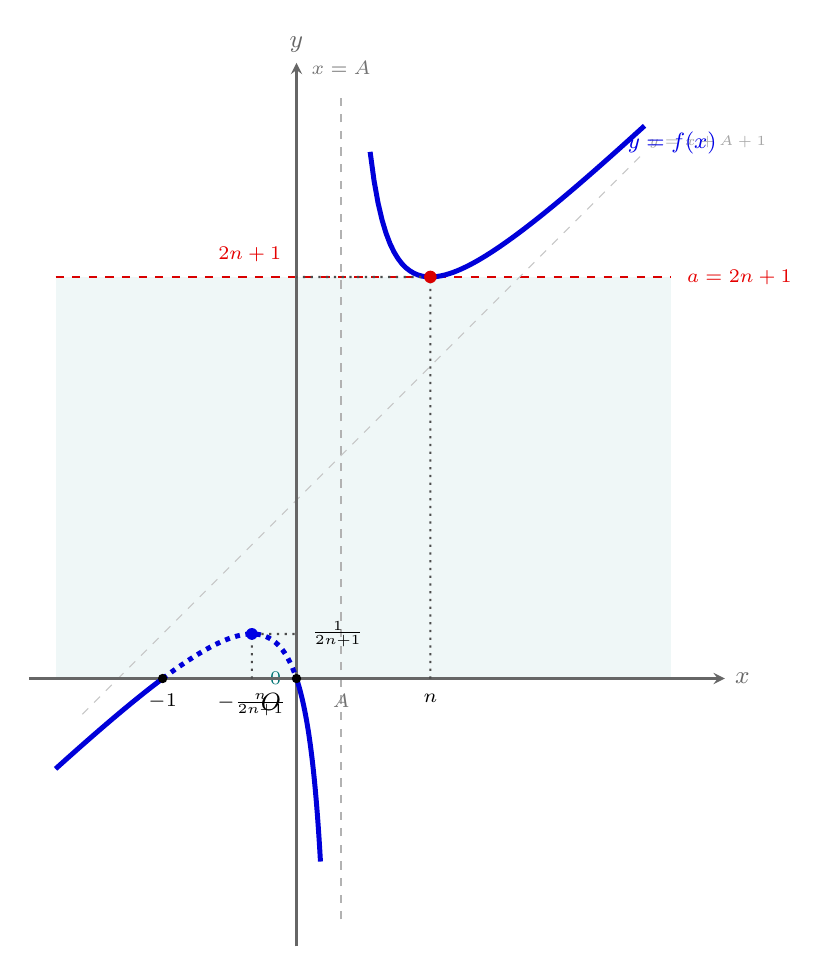
\begin{tikzpicture}[scale=1.7, >=stealth, every node/.style={font=\small}]

    % --- 1. n = 1 に基づく厳密な座標パラメータ ---
    % n = 1
    % A = 1/3 ≈ 0.3333
    % 極小点: (n, 2n+1) = (1, 3)
    % 極大点: (-1/3, 1/3) = (-0.3333, 0.3333)
    \pgfmathsetmacro{\nVal}{1.0}
    \pgfmathsetmacro{\valA}{1.0 / 3.0}           % A = 1/3
    \pgfmathsetmacro{\xMin}{\nVal}               % x = 1
    \pgfmathsetmacro{\yMin}{2.0*\nVal + 1.0}     % y = 3 (厳密一致)
    \pgfmathsetmacro{\xMax}{-\nVal / (2.0*\nVal + 1.0)} % -1/3
    \pgfmathsetmacro{\yMax}{1.0 / (2.0*\nVal + 1.0)}    % 1/3

    \coordinate (O)      at (0, 0);
    \coordinate (Pt_min) at (\xMin, \yMin);
    \coordinate (Pt_max) at (\xMax, \yMax);

    % --- 2. y = a の許容帯 0 < a < 2n+1 (= 3) の塗りつぶし ---
    \fill[teal!8, opacity=0.8] (-1.8, 0) rectangle (2.8, \yMin);

    % 許容帯の境界線 (a = 2n+1 = 3, a = 0)
    \draw[thick, dashed, red!85!black] (-1.8, \yMin) -- (2.8, \yMin)
    node[right=2pt, font=\scriptsize, red!90!black] {$a = 2n+1$};
    \draw[thick, dashed, teal!85!black] (-1.8, 0) -- (2.8, 0);
    \node[above left=2pt, font=\scriptsize, red!90!black] at (0, \yMin) {$2n+1$};
    \node[left=2pt, font=\scriptsize, teal!90!black] at (0, 0) {$0$};

    % --- 3. 漸近線 ---
    % (i) 垂直漸近線 x = A (= 1/3)
    \draw[dashed, gray!60, thick] (\valA, -1.8) -- (\valA, 4.4);
    \node[above=2pt, font=\scriptsize, gray!90!black] at (\valA, 4.4) {$x = A$};
    \node[below=2pt, font=\scriptsize, gray!90!black] at (\valA, 0) {$A$};

    % (ii) 斜め漸近線 y = x + A + 1 = x + 4/3
    \draw[dashed, gray!45, thin, domain=-1.6:2.6]
    plot (\x, {\x + \valA + 1.0})
    node[above right=-2pt, font=\tiny, gray!70] {$y = x + A + 1$};

    % --- 4. 座標軸 ---
    \draw[->, thick, gray!80!black] (-2.0, 0) -- (3.2, 0) node[right] {$x$};
    \draw[->, thick, gray!80!black] (0, -2.0) -- (0, 4.6) node[above] {$y$};
    \node[below left=2pt] at (O) {$O$};

    % --- 5. 双曲線 y = f(x) の厳密プロット ---
    % f(x) = (x^2 + x)/(x - 1/3)
    % (i) 左側の分枝 (x < 1/3)
    \draw[line width=1.8pt, blue!85!black, domain=-1.8:-1.0, samples=70]
    plot (\x, {(\x*\x + \x)/(\x - \valA)});
    % (i) 左側の分枝 (x < 1/3)
    \draw[line width=1.8pt, blue!85!black, domain=0:0.18, samples=70]
    plot (\x, {(\x*\x + \x)/(\x - \valA)});
    % (i) 左側の分枝 (x < 1/3)
    \draw[line width=1.8pt, blue!85!black, domain=-1.0:0, samples=70, dotted]
    plot (\x, {(\x*\x + \x)/(\x - \valA)});
    % (ii) 右側の分枝 (x > 1/3)
    \draw[line width=1.8pt, blue!85!black, domain=0.55:2.6, samples=70]
    plot (\x, {(\x*\x + \x)/(\x - \valA)});
    \node[blue!90!black, font=\footnotesize\bfseries, right] at (2.4, 4.0)
    {$y = f(x)$};

    % --- 6. 主要点のプロットと投影破線 ---
    % x 切片 (-1, 0) と原点 (0, 0)
    \node[circle, fill, inner sep=1.2pt] at (-1.0, 0) {}; \node[below=2pt, font=\scriptsize] at (-1.0, 0) {$-1$};
    \node[circle, fill, inner sep=1.2pt] at (O) {};

    % 極大点 (-n/(2n+1), 1/(2n+1)) = (-1/3, 1/3)
    \draw[thick, dotted, gray!60!black] (\xMax, 0) -- (Pt_max) -- (0, \yMax);
    \node[circle, fill=blue!90!black, inner sep=1.5pt] at (Pt_max) {};
    \node[below=2pt, font=\scriptsize] at (\xMax, 0) {$-\frac{n}{2n+1}$};
    \node[right=2pt, font=\scriptsize]  at (0, \yMax) {$\frac{1}{2n+1}$};

    % 極小点 (n, 2n+1) = (1, 3) (厳密に接する)
    \draw[thick, dotted, gray!60!black] (\xMin, 0) -- (Pt_min) -- (0, \yMin);
    \node[circle, fill=red!85!black, inner sep=1.6pt] at (Pt_min) {};
    \node[below=2pt, font=\scriptsize] at (\xMin, 0) {$n$};
    % \node[above=2pt, font=\tiny, red!90!black] at (Pt_min) {極小 $(n, 2n+1)$};

  \end{tikzpicture}
  \caption{$y = f(x)$ のグラフと極小値 $f(n) = 2n+1$ および許容範囲 $0 < a < 2n+1$}
  \label{fig:fx_hyperbola_parameter_a_exact}
\end{figure}

このグラフから，\cref{eq:5}の条件が成り立つ$a$の条件は$m$が整数であることに注意して
\begin{align}
  0 < a < 2n+1
\end{align}
である．

{\bf [別解]}

本解答と同じく$A=\dfrac{n^2}{2n+1}$として
\begin{align}
  f(x) = x^2 - (a-1)x + Aa
\end{align}
に対して$f(m)>0$となる条件を考える．

$f(x)=0$ の判別式 $D$ として
\begin{align}
  D &= (a-1)^2 - 4Aa \\
  &= a^2 - 2(1+2A)a + 1
\end{align}
である．$f(x)=0$が解を持つかどうかで場合分けして考える．

まず$f(x)=0$が解を持たないときは$f(x)>0$となって自明に条件を満たす．この時は
\begin{align}
  D < 0
  & \iff (1+2A) - \sqrt{4A^2+4A} < a < (1+2A) + \sqrt{4A^2+4A} \\
  & \iff \dfrac{1}{2n+1} < a < 2n+1 \label{eq:6}
\end{align}
である．

$f(x)=0$が解を持つ時，すなわち\cref{eq:6}以外の時，
$f(x)=0$の解は
\begin{align}
  x
  &= \dfrac{1}{2}\left[ (a-1) \pm \sqrt{(a-1)^2 - 4Aa} \right] \\
  &= \dfrac{1}{2}\left[ (a-1) \pm \sqrt{a^2 - 2(1+2A)a + 1} \right]
\end{align}
である．これらを $\alpha, \beta$ ($\alpha \le \beta$) とする．

\subparagraph{$1^\circ \ 0 < a \le \dfrac{1}{2n+1}$ の時}

この時，$\alpha$と$-1$の大小を比較すると
\begin{align}
  \alpha &= \dfrac{1}{2}\left[ (a-1) - \sqrt{a^2-2(1+2A)a+1} \right] > -1
\end{align}
\begin{align}
  &\iff (a+1)^2 > a^2 - 2(1+2A)a + 1 \\
  &\iff 2(1+A)a > 0 \label{eq:7}
\end{align}
である．\cref{eq:7}は成立するので $\alpha > -1$ である．
同様に $\beta < 0$ だから， $-1 < \alpha < \beta < 0$である．
したがって任意の $m \in \mathbb{Z}$ に対し $f(m) > 0$である．

\subparagraph{$2^\circ \ 2n+1 \le a$の時}

この時は具体的に$x=n \in \mathbb{N}$とすると
\begin{align}
  f(n) &= (A-n)a + n^2 + n \\
  &= \dfrac{-(n^2+n)}{2n+1} a + n^2 + n \le 0
\end{align}
だから不適である．
\casesend

以上まとめて求める条件は $0 < a < 2n+1$ である．

\newpage

\end{document}
